
%% bare_conf.tex
%% V1.3
%% 2007/01/11
%% by Michael Shell
%% See:
%% http://www.michaelshell.org/
%% for current contact information.
%%
%% This is a skeleton file demonstrating the use of IEEEtran.cls
%% (requires IEEEtran.cls version 1.7 or later) with an IEEE conference paper.
%%
%% Support sites:
%% http://www.michaelshell.org/tex/ieeetran/
%% http://www.ctan.org/tex-archive/macros/latex/contrib/IEEEtran/
%% and
%% http://www.ieee.org/

%%*************************************************************************
%% Legal Notice:
%% This code is offered as-is without any warranty either expressed or
%% implied; without even the implied warranty of MERCHANTABILITY or
%% FITNESS FOR A PARTICULAR PURPOSE! 
%% User assumes all risk.
%% In no event shall IEEE or any contributor to this code be liable for
%% any damages or losses, including, but not limited to, incidental,
%% consequential, or any other damages, resulting from the use or misuse
%% of any information contained here.
%%
%% All comments are the opinions of their respective authors and are not
%% necessarily endorsed by the IEEE.
%%
%% This work is distributed under the LaTeX Project Public License (LPPL)
%% ( http://www.latex-project.org/ ) version 1.3, and may be freely used,
%% distributed and modified. A copy of the LPPL, version 1.3, is included
%% in the base LaTeX documentation of all distributions of LaTeX released
%% 2003/12/01 or later.
%% Retain all contribution notices and credits.
%% ** Modified files should be clearly indicated as such, including  **
%% ** renaming them and changing author support contact information. **
%%
%% File list of work: IEEEtran.cls, IEEEtran_HOWTO.pdf, bare_adv.tex,
%%                    bare_conf.tex, bare_jrnl.tex, bare_jrnl_compsoc.tex
%%*************************************************************************

% *** Authors should verify (and, if needed, correct) their LaTeX system  ***
% *** with the testflow diagnostic prior to trusting their LaTeX platform ***
% *** with production work. IEEE's font choices can trigger bugs that do  ***
% *** not appear when using other class files.                            ***
% The testflow support page is at:
% http://www.michaelshell.org/tex/testflow/



% Note that the a4paper option is mainly intended so that authors in
% countries using A4 can easily print to A4 and see how their papers will
% look in print - the typesetting of the document will not typically be
% affected with changes in paper size (but the bottom and side margins will).
% Use the testflow package mentioned above to verify correct handling of
% both paper sizes by the user's LaTeX system.
%
% Also note that the "draftcls" or "draftclsnofoot", not "draft", option
% should be used if it is desired that the figures are to be displayed in
% draft mode.
%
\documentclass[10pt, conference, compsocconf]{IEEEtran}
% Add the compsocconf option for Computer Society conferences.
%
% If IEEEtran.cls has not been installed into the LaTeX system files,
% manually specify the path to it like:
% \documentclass[conference]{../sty/IEEEtran}





% Some very useful LaTeX packages include:
% (uncomment the ones you want to load)


% *** MISC UTILITY PACKAGES ***
%
%\usepackage{ifpdf}
% Heiko Oberdiek's ifpdf.sty is very useful if you need conditional
% compilation based on whether the output is pdf or dvi.
% usage:
% \ifpdf
%   % pdf code
% \else
%   % dvi code
% \fi
% The latest version of ifpdf.sty can be obtained from:
% http://www.ctan.org/tex-archive/macros/latex/contrib/oberdiek/
% Also, note that IEEEtran.cls V1.7 and later provides a builtin
% \ifCLASSINFOpdf conditional that works the same way.
% When switching from latex to pdflatex and vice-versa, the compiler may
% have to be run twice to clear warning/error messages.






% *** CITATION PACKAGES ***
%
%\usepackage{cite}
% cite.sty was written by Donald Arseneau
% V1.6 and later of IEEEtran pre-defines the format of the cite.sty package
% \cite{} output to follow that of IEEE. Loading the cite package will
% result in citation numbers being automatically sorted and properly
% "compressed/ranged". e.g., [1], [9], [2], [7], [5], [6] without using
% cite.sty will become [1], [2], [5]--[7], [9] using cite.sty. cite.sty's
% \cite will automatically add leading space, if needed. Use cite.sty's
% noadjust option (cite.sty V3.8 and later) if you want to turn this off.
% cite.sty is already installed on most LaTeX systems. Be sure and use
% version 4.0 (2003-05-27) and later if using hyperref.sty. cite.sty does
% not currently provide for hyperlinked citations.
% The latest version can be obtained at:
% http://www.ctan.org/tex-archive/macros/latex/contrib/cite/
% The documentation is contained in the cite.sty file itself.






% *** GRAPHICS RELATED PACKAGES ***
%
\ifCLASSINFOpdf
  % \usepackage[pdftex]{graphicx}
  % declare the path(s) where your graphic files are
  % \graphicspath{{../pdf/}{../jpeg/}}
  % and their extensions so you won't have to specify these with
  % every instance of \includegraphics
  % \DeclareGraphicsExtensions{.pdf,.jpeg,.png}
\else
  % or other class option (dvipsone, dvipdf, if not using dvips). graphicx
  % will default to the driver specified in the system graphics.cfg if no
  % driver is specified.
  % \usepackage[dvips]{graphicx}
  % declare the path(s) where your graphic files are
  % \graphicspath{{../eps/}}
  % and their extensions so you won't have to specify these with
  % every instance of \includegraphics
  % \DeclareGraphicsExtensions{.eps}
\fi
% graphicx was written by David Carlisle and Sebastian Rahtz. It is
% required if you want graphics, photos, etc. graphicx.sty is already
% installed on most LaTeX systems. The latest version and documentation can
% be obtained at: 
% http://www.ctan.org/tex-archive/macros/latex/required/graphics/
% Another good source of documentation is "Using Imported Graphics in
% LaTeX2e" by Keith Reckdahl which can be found as epslatex.ps or
% epslatex.pdf at: http://www.ctan.org/tex-archive/info/
%
% latex, and pdflatex in dvi mode, support graphics in encapsulated
% postscript (.eps) format. pdflatex in pdf mode supports graphics
% in .pdf, .jpeg, .png and .mps (metapost) formats. Users should ensure
% that all non-photo figures use a vector format (.eps, .pdf, .mps) and
% not a bitmapped formats (.jpeg, .png). IEEE frowns on bitmapped formats
% which can result in "jaggedy"/blurry rendering of lines and letters as
% well as large increases in file sizes.
%
% You can find documentation about the pdfTeX application at:
% http://www.tug.org/applications/pdftex





% *** MATH PACKAGES ***
%
%\usepackage[cmex10]{amsmath}
% A popular package from the American Mathematical Society that provides
% many useful and powerful commands for dealing with mathematics. If using
% it, be sure to load this package with the cmex10 option to ensure that
% only type 1 fonts will utilized at all point sizes. Without this option,
% it is possible that some math symbols, particularly those within
% footnotes, will be rendered in bitmap form which will result in a
% document that can not be IEEE Xplore compliant!
%
% Also, note that the amsmath package sets \interdisplaylinepenalty to 10000
% thus preventing page breaks from occurring within multiline equations. Use:
%\interdisplaylinepenalty=2500
% after loading amsmath to restore such page breaks as IEEEtran.cls normally
% does. amsmath.sty is already installed on most LaTeX systems. The latest
% version and documentation can be obtained at:
% http://www.ctan.org/tex-archive/macros/latex/required/amslatex/math/





% *** SPECIALIZED LIST PACKAGES ***
%
%\usepackage{algorithmic}
% algorithmic.sty was written by Peter Williams and Rogerio Brito.
% This package provides an algorithmic environment fo describing algorithms.
% You can use the algorithmic environment in-text or within a figure
% environment to provide for a floating algorithm. Do NOT use the algorithm
% floating environment provided by algorithm.sty (by the same authors) or
% algorithm2e.sty (by Christophe Fiorio) as IEEE does not use dedicated
% algorithm float types and packages that provide these will not provide
% correct IEEE style captions. The latest version and documentation of
% algorithmic.sty can be obtained at:
% http://www.ctan.org/tex-archive/macros/latex/contrib/algorithms/
% There is also a support site at:
% http://algorithms.berlios.de/index.html
% Also of interest may be the (relatively newer and more customizable)
% algorithmicx.sty package by Szasz Janos:
% http://www.ctan.org/tex-archive/macros/latex/contrib/algorithmicx/




% *** ALIGNMENT PACKAGES ***
%
%\usepackage{array}
% Frank Mittelbach's and David Carlisle's array.sty patches and improves
% the standard LaTeX2e array and tabular environments to provide better
% appearance and additional user controls. As the default LaTeX2e table
% generation code is lacking to the point of almost being broken with
% respect to the quality of the end results, all users are strongly
% advised to use an enhanced (at the very least that provided by array.sty)
% set of table tools. array.sty is already installed on most systems. The
% latest version and documentation can be obtained at:
% http://www.ctan.org/tex-archive/macros/latex/required/tools/


%\usepackage{mdwmath}
%\usepackage{mdwtab}
% Also highly recommended is Mark Wooding's extremely powerful MDW tools,
% especially mdwmath.sty and mdwtab.sty which are used to format equations
% and tables, respectively. The MDWtools set is already installed on most
% LaTeX systems. The lastest version and documentation is available at:
% http://www.ctan.org/tex-archive/macros/latex/contrib/mdwtools/


% IEEEtran contains the IEEEeqnarray family of commands that can be used to
% generate multiline equations as well as matrices, tables, etc., of high
% quality.

\usepackage[ruled,linesnumbered,lined]{algorithm2e}

%\usepackage{amsmath}
%\usepackage{enumitem}
%\usepackage{eqparbox}
% Also of notable interest is Scott Pakin's eqparbox package for creating
% (automatically sized) equal width boxes - aka "natural width parboxes".
% Available at:
% http://www.ctan.org/tex-archive/macros/latex/contrib/eqparbox/

\usepackage{graphicx}
\usepackage{subfigure}
\graphicspath{{figure/}}

\usepackage{hyperref}
\usepackage{multirow}
\usepackage{balance}
\usepackage{comment}
\usepackage{tikz}
\usepackage[numbers,sort&compress]{natbib}

\usepackage{color}
\definecolor{dkgreen}{rgb}{0,0.6,0}
\definecolor{gray}{rgb}{0.5,0.5,0.5}
\definecolor{mauve}{rgb}{0.58,0,0.82}
% Default settings for code listings

\newcommand{\tabincell}[2]{\begin{tabular}{@{}#1@{}}#2\end{tabular}}

\def\sharedaffiliation{
\end{tabular}
\begin{tabular}{c}}

% *** SUBFIGURE PACKAGES ***
%\usepackage[tight,footnotesize]{subfigure}
% subfigure.sty was written by Steven Douglas Cochran. This package makes it
% easy to put subfigures in your figures. e.g., "Figure 1a and 1b". For IEEE
% work, it is a good idea to load it with the tight package option to reduce
% the amount of white space around the subfigures. subfigure.sty is already
% installed on most LaTeX systems. The latest version and documentation can
% be obtained at:
% http://www.ctan.org/tex-archive/obsolete/macros/latex/contrib/subfigure/
% subfigure.sty has been superceeded by subfig.sty.

%\usepackage[caption=false]{caption}
%\usepackage[font=footnotesize]{subfig}
% subfig.sty, also written by Steven Douglas Cochran, is the modern
% replacement for subfigure.sty. However, subfig.sty requires and
% automatically loads Axel Sommerfeldt's caption.sty which will override
% IEEEtran.cls handling of captions and this will result in nonIEEE style
% figure/table captions. To prevent this problem, be sure and preload
% caption.sty with its "caption=false" package option. This is will preserve
% IEEEtran.cls handing of captions. Version 1.3 (2005/06/28) and later 
% (recommended due to many improvements over 1.2) of subfig.sty supports
% the caption=false option directly:
%\usepackage[caption=false,font=footnotesize]{subfig}
%
% The latest version and documentation can be obtained at:
% http://www.ctan.org/tex-archive/macros/latex/contrib/subfig/
% The latest version and documentation of caption.sty can be obtained at:
% http://www.ctan.org/tex-archive/macros/latex/contrib/caption/




% *** FLOAT PACKAGES ***
%
%\usepackage{fixltx2e}
% fixltx2e, the successor to the earlier fix2col.sty, was written by
% Frank Mittelbach and David Carlisle. This package corrects a few problems
% in the LaTeX2e kernel, the most notable of which is that in current
% LaTeX2e releases, the ordering of single and double column floats is not
% guaranteed to be preserved. Thus, an unpatched LaTeX2e can allow a
% single column figure to be placed prior to an earlier double column
% figure. The latest version and documentation can be found at:
% http://www.ctan.org/tex-archive/macros/latex/base/



%\usepackage{stfloats}
% stfloats.sty was written by Sigitas Tolusis. This package gives LaTeX2e
% the ability to do double column floats at the bottom of the page as well
% as the top. (e.g., "\begin{figure*}[!b]" is not normally possible in
% LaTeX2e). It also provides a command:
%\fnbelowfloat
% to enable the placement of footnotes below bottom floats (the standard
% LaTeX2e kernel puts them above bottom floats). This is an invasive package
% which rewrites many portions of the LaTeX2e float routines. It may not work
% with other packages that modify the LaTeX2e float routines. The latest
% version and documentation can be obtained at:
% http://www.ctan.org/tex-archive/macros/latex/contrib/sttools/
% Documentation is contained in the stfloats.sty comments as well as in the
% presfull.pdf file. Do not use the stfloats baselinefloat ability as IEEE
% does not allow \baselineskip to stretch. Authors submitting work to the
% IEEE should note that IEEE rarely uses double column equations and
% that authors should try to avoid such use. Do not be tempted to use the
% cuted.sty or midfloat.sty packages (also by Sigitas Tolusis) as IEEE does
% not format its papers in such ways.





% *** PDF, URL AND HYPERLINK PACKAGES ***
%
%\usepackage{url}
% url.sty was written by Donald Arseneau. It provides better support for
% handling and breaking URLs. url.sty is already installed on most LaTeX
% systems. The latest version can be obtained at:
% http://www.ctan.org/tex-archive/macros/latex/contrib/misc/
% Read the url.sty source comments for usage information. Basically,
% \url{my_url_here}.





% *** Do not adjust lengths that control margins, column widths, etc. ***
% *** Do not use packages that alter fonts (such as pslatex).         ***
% There should be no need to do such things with IEEEtran.cls V1.6 and later.
% (Unless specifically asked to do so by the journal or conference you plan
% to submit to, of course. )


% correct bad hyphenation here
\hyphenation{op-tical net-works semi-conduc-tor}


\begin{document}
%
% paper title
% can use linebreaks \\ within to get better formatting as desired
\title{A Performance Analytical Model based on Decision Tree in GPU Architectures}


% author names and affiliations
% use a multiple column layout for up to two different
% affiliations

\author{\IEEEauthorblockN{First Author, Second Author, Hai Jin}
\IEEEauthorblockA{Services Computing Technology and System Lab\\
Cluster and Grid Computing Lab\\
Big Data Technology and System Lab\\
School of Computer Science and Technology\\
Huazhong University of Science and Technology, Wuhan, 430074, China\\
Email: \{first, second, haijin\}@hust.edu.cn}
}

% conference papers do not typically use \thanks and this command
% is locked out in conference mode. If really needed, such as for
% the acknowledgment of grants, issue a \IEEEoverridecommandlockouts
% after \documentclass

% for over three affiliations, or if they all won't fit within the width
% of the page, use this alternative format:
% 
%\author{\IEEEauthorblockN{Michael Shell\IEEEauthorrefmark{1},
%Homer Simpson\IEEEauthorrefmark{2},
%James Kirk\IEEEauthorrefmark{3}, 
%Montgomery Scott\IEEEauthorrefmark{3} and
%Eldon Tyrell\IEEEauthorrefmark{4}}
%\IEEEauthorblockA{\IEEEauthorrefmark{1}School of Electrical and Computer Engineering\\
%Georgia Institute of Technology,
%Atlanta, Georgia 30332--0250\\ Email: see http://www.michaelshell.org/contact.html}
%\IEEEauthorblockA{\IEEEauthorrefmark{2}Twentieth Century Fox, Springfield, USA\\
%Email: homer@thesimpsons.com}
%\IEEEauthorblockA{\IEEEauthorrefmark{3}Starfleet Academy, San Francisco, California 96678-2391\\
%Telephone: (800) 555--1212, Fax: (888) 555--1212}
%\IEEEauthorblockA{\IEEEauthorrefmark{4}Tyrell Inc., 123 Replicant Street, Los Angeles, California 90210--4321}}




% use for special paper notices
%\IEEEspecialpapernotice{(Invited Paper)}




% make the title area
\maketitle


\begin{abstract}
%In-memory computing systems are shown to suffer serious memory pressure as well as they are for service, the memory pressure will effect all submitted jobs. Memory pressure is coming from the running tasks as they produce massive long-lived data objects in limited memory, which brings significant memory and CPU overheads. Some tasks result in heavy memory pressure because of the operations and dataset they process, which affects all running tasks in the system. We find that each task includes several function APIs provided by the framework, and most function APIs produce long-lived data objects in memory within their own regular models; some need constant memory space while some need linear memory space. As different models have different impact on memory pressure, we propose memory usage rate to classify which model a task belongs to. Based on the memory usage rate, we design a scheduler called MURS to schedule all running tasks and mitigate heavy memory pressure. We implement MURS in Spark and the experimental study shows that, when compare to Spark, our scheduler can 1) decrease the execution time of submitted job by up to 65.8\%; 2) mitigate the memory pressure in server by decreasing the garbage collection time by up to 81\%; and 3) avoid about 90\% of spill tasks to reduce disk I/O.

Good Good Study, Day Day Up. Wish!

\end{abstract}

\begin{IEEEkeywords}
performance analysis; GPU architectures; decision tree; analytical model

\end{IEEEkeywords}


% For peer review papers, you can put extra information on the cover
% page as needed:
% \ifCLASSOPTIONpeerreview
% \begin{center} \bfseries EDICS Category: 3-BBND \end{center}
% \fi
%
% For peerreview papers, this IEEEtran command inserts a page break and
% creates the second title. It will be ignored for other modes.
\IEEEpeerreviewmaketitle

\section{Introduction}

Background(一段) 

\begin{itemize}
\item 1. GPU性能评估的重要性;
\item 2. GPU性能评估需要考虑的问题,准确性,指导性等等。
\end{itemize}

Motivation(一段) 

\begin{itemize}
\item 1. 监控工具可以监控的指标有非常多种,需要熟练的技术知识才能分析这些指标;
\item 2. 指标太多不利于直接发现最关键的性能瓶颈,
需要一定的经验知识作为辅导;
\item 3. 数学模型的建立有助于评估性能,但是精确的模型的建立及理解都很困难,对模型建立者和使用者都需要对GPU架构有深刻理解。
\end{itemize}

Introduction(两段) 

监控工具得到的指标非常多,往往一个指标或者多个指标集可以指向一个具体的性能问题。而不同的GPU程序又必然有一个影响最大的性能瓶颈。所以能够快速定位影响最大的性能瓶颈非常关键。决策树的分析模型是机器学习中基于信息论的分类模型,更加专注于信息对整个数据集的影响,因此由决策树决定需要考虑的指标,非常适合解决该问题。

获取影响最大的指标集后,极大地缩小了需要考虑的范围。如果继续采用决策树的分类性能瓶颈和优化方案具有一定的误差,这与机器学习特性有关。传统的数学模型准确度往往比机器学习算法准确率要高,由于需要考虑的指标集已经很小了,因此通过理论模型分析这些指标更为恰当。分析方法从三个层面考虑:应用层面(包括应用在计算需求、数据排列上的处理),系统层面(包括指令调度、资源管理和分配等),硬件层面(包括通信带宽、资源特性等)。结合小范围的数据集和三个层面,本文模型可以快速定位并准确提出性能瓶颈与优化方案。

Contribution(三点) 

\begin{itemize}
\item 1. 提供了一种结合决策树模型和理论分析模型的GPU应用性能分析模型,可以更加准确地定位性能瓶颈并提出优化方案。
\item 2. 提供了一种基于决策树的分析算法,在GPU应用程序的监控数据中,由决策树决定影响最大的指标集并做进一步的理论分析。决策树的方法可以快速地决策GPU应用程序的瓶颈,缩小需要考虑和分析的范围。决策树不仅基于microbenchmark,还可以基于上层数据处理系统的benchmark训练,适用范围广。
\item 3. 基于决策树的分析结果,提出了面向应用、系统和硬件的三层理论分析模型,进一步定位决策树得出的瓶颈结果。理论分析模型可以在小范围内更加准确地确定GPU应用瓶颈并提出优化方法。
\end{itemize}

Paper(一段) 

第II章,相关工作;第III章:背景;第IV章,决策树;第V章,分析模型;第VI章,实验;第VII章,结论。
%\section{Motivation}
\label{sec:motivation}

Memory is a critical type of resource in current data processing systems, especially in the in-memory computing systems~\cite{shi:mammoth}. However, limited memory space leads to memory pressure and can cause frequent garbage collection or out-of-memory errors~\cite{fang2015interruptible}, both of which seriously affect the performance of the data processing system. A data processing system is often deployed as a service. To understand the impact of memory pressure on the data processing systems and identify the cause of inefficiency, we investigate the running of the tasks with different memory requirements. We choose two types of applications, PageRank(PR) and WordCount(WC), which are the common benchmarks in Spark. The input dataset of PR and WC are webbase-2001 (30GB) and HiBench Random Writer (50GB). As a data processing system, Spark can also work as a server through Spark Job Server. We first run the tasks in the service mode, in which we submit PR and WC simultaneously to the Spark server and run them with a fair scheduler in Spark. As a comparison, we also run PR and WC in the batch mode, in which PR and WC are processed one after the other. We record the execution times and garbage collections times of all tasks under these two modes, which are plotted in Figure~\ref{fig:memorypressure}. We then analyze the memory pressure through the results. 

%Memory is an important resource in current data processing systems, especially in these in-memory computing systems~\cite{shi:mammoth}. Limited memory space will result in memory pressure. The impact of memory pressure can be frequent garbage collection~\cite{lulu:deca} or out of memory error~\cite{fang2015interruptible}, both have serious effect on the data processing system. We can evaluate the memory pressure by PageRank(PR) and WordCount(WC), two common benchmarks, in Spark. The details of clusters and applications are shown in the evaluation. Spark can work for service by Spark Job Server. We firstly run PR and WC individually in batch processing to evaluate the memory pressure themselves, and then evaluate the memory pressure in Spark for service by submitting them together to Spark Job Server. In each stage, we count the medium of execution time and garbage collection time of all tasks, as shown in Figure~\ref{fig:memorypressure}.

\begin{figure}[!t]
\centering
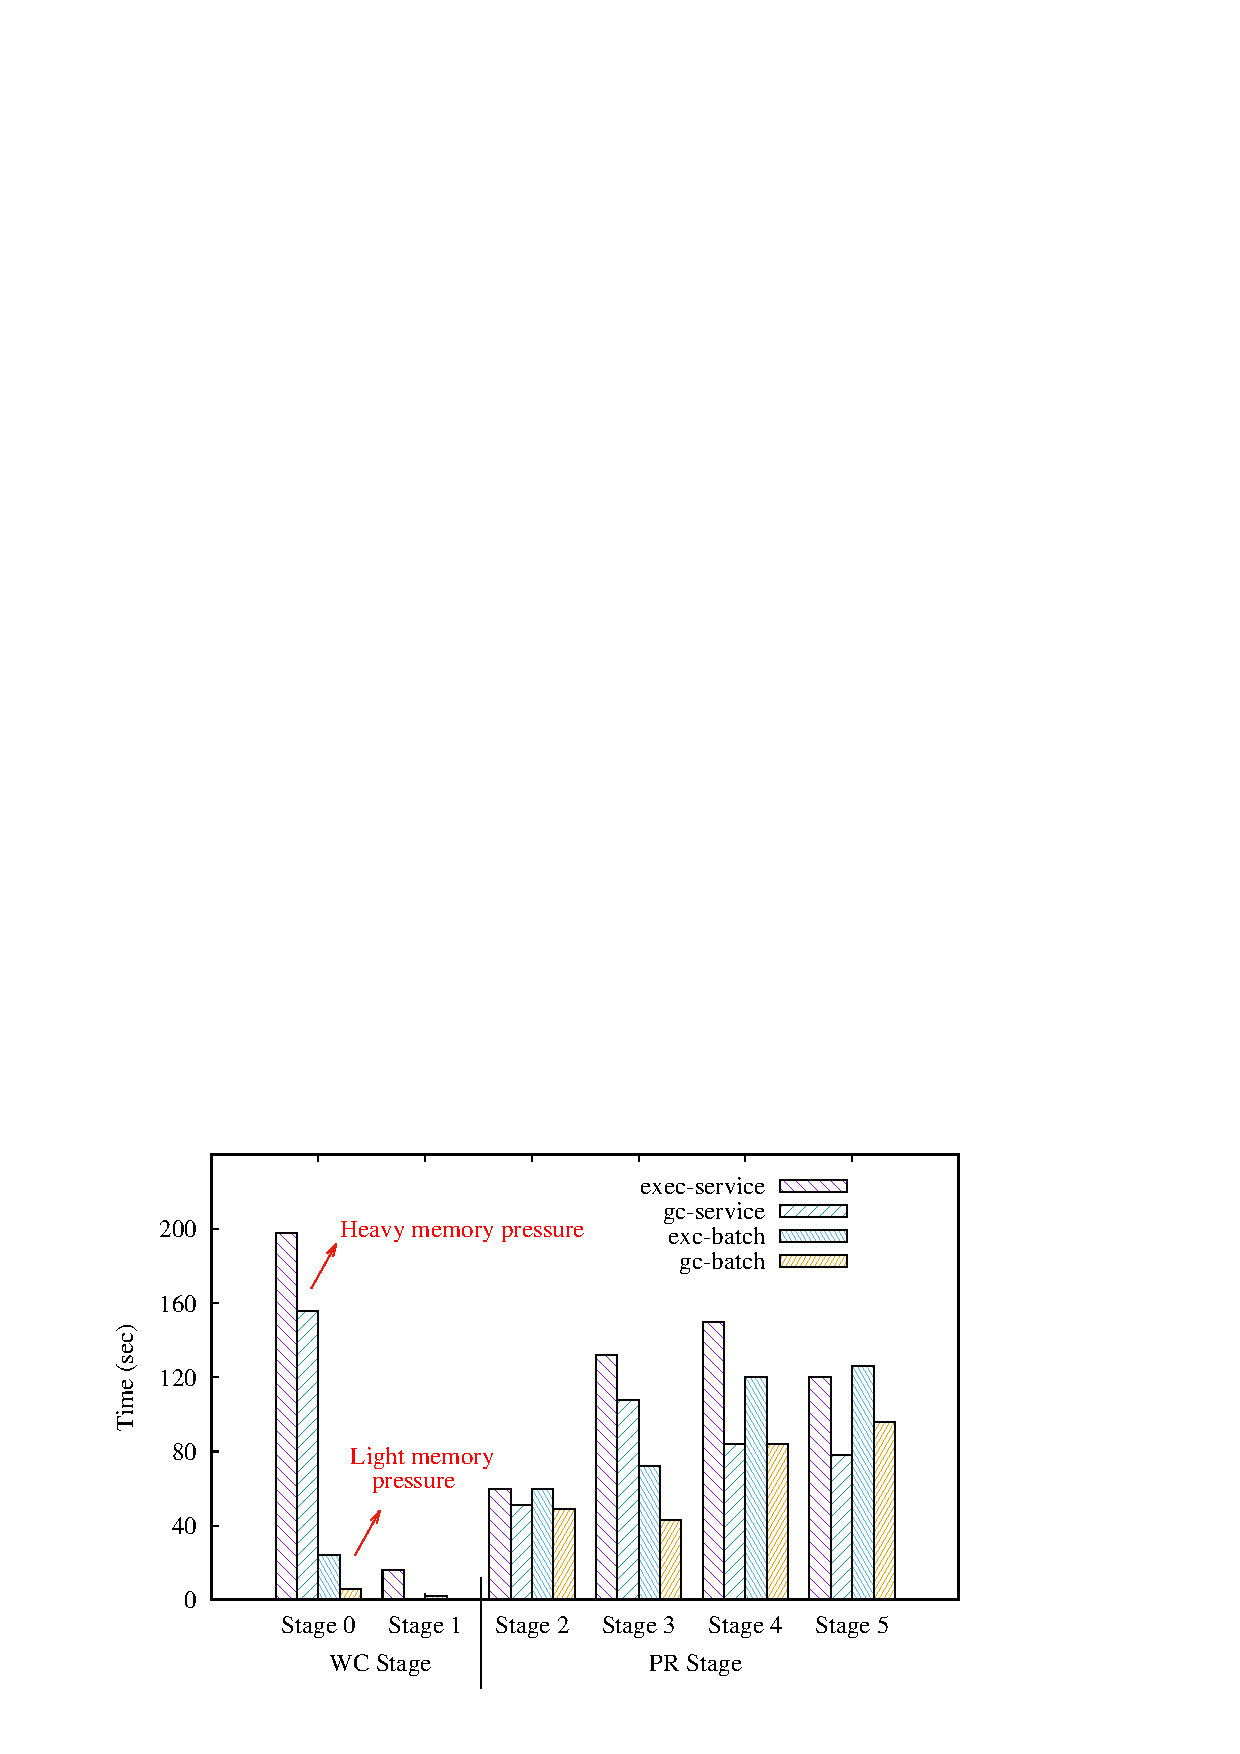
\includegraphics[width=0.4\textwidth]{motivation-exec-gc.pdf}
\vspace{-2mm}
\caption{WC suffers memory pressure from PR}
\vspace{-6mm}
\label{fig:memorypressure}
\end{figure}

\begin{comment}
\begin{figure}[!t]
\centering
\subfigure[Execution Time]{
\label{fig:subfig:mot-exec}
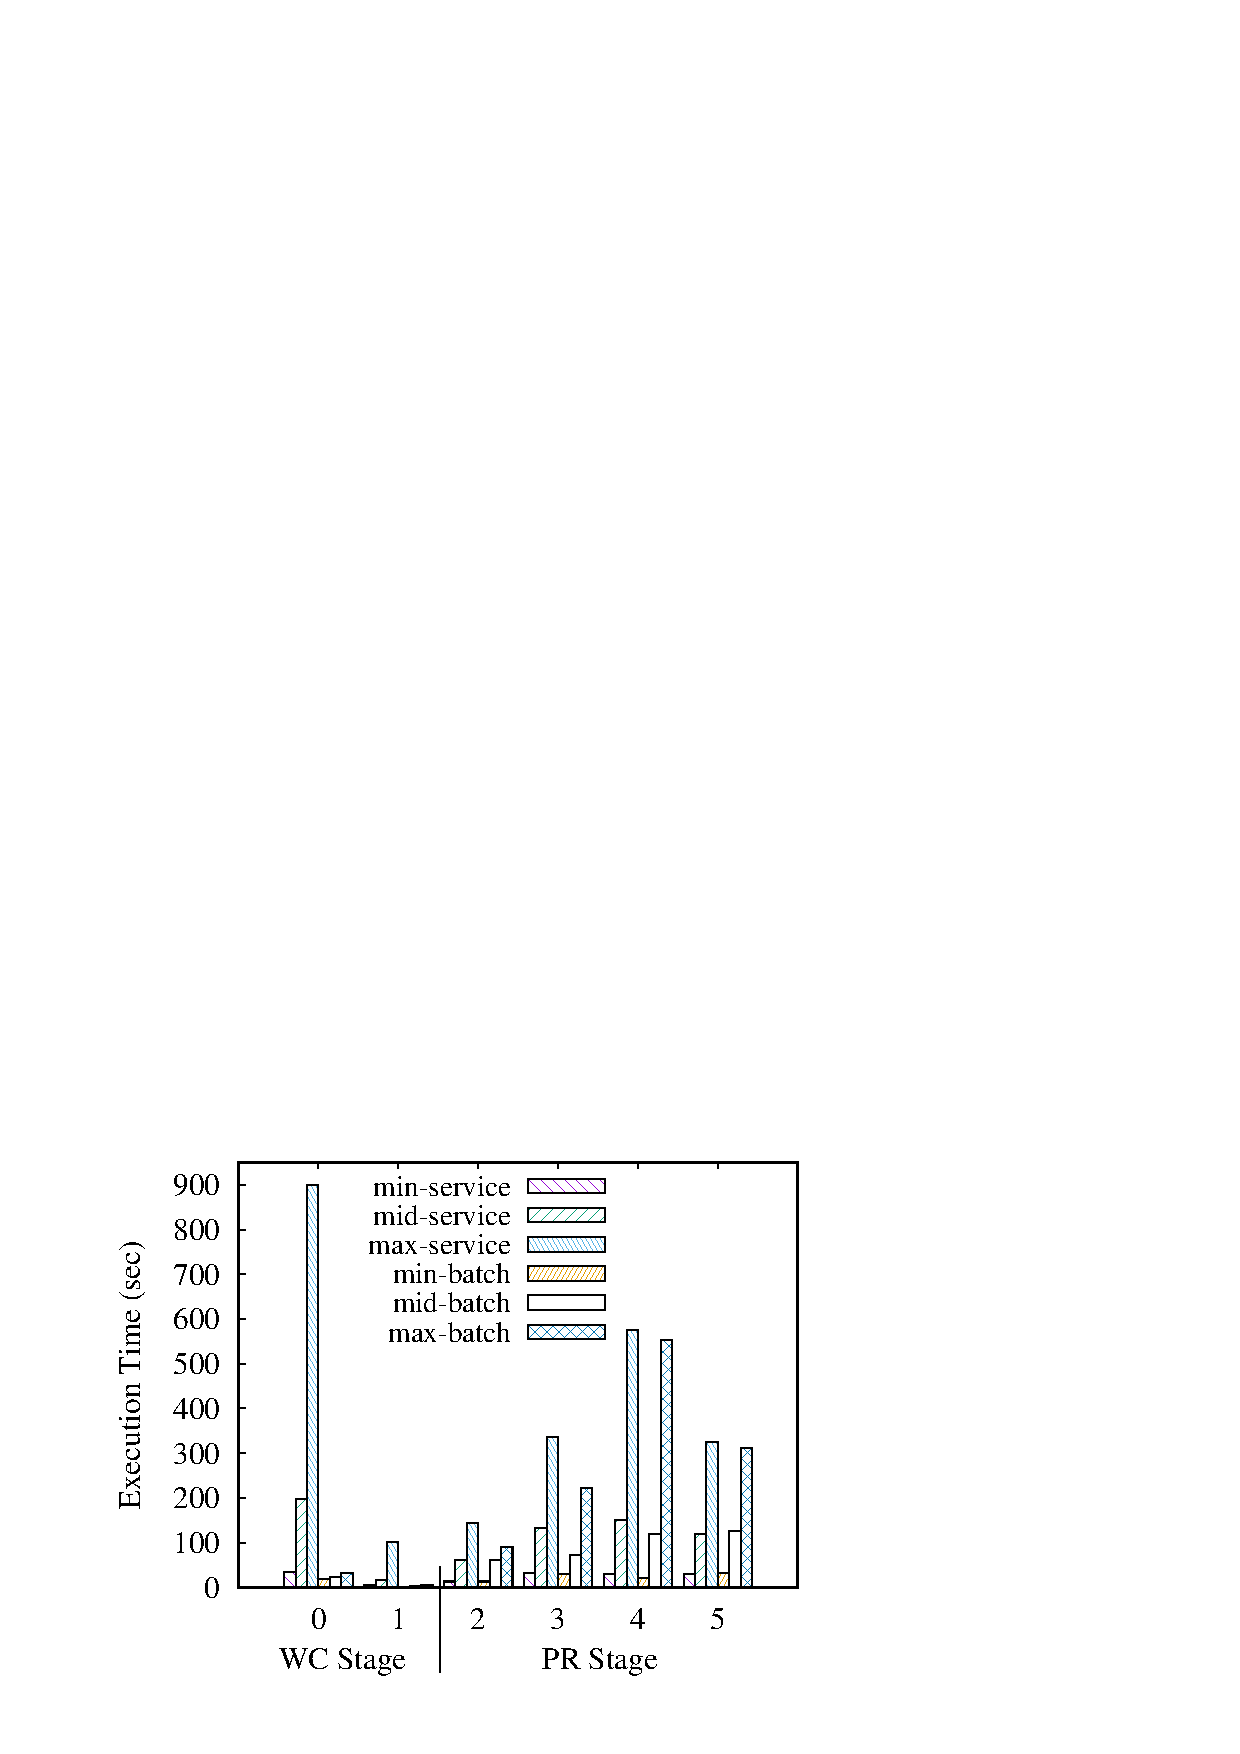
\includegraphics[width=0.231\textwidth]{motivation-exec.pdf}}
\hspace{-1.3ex}
\subfigure[GC Time]{
\label{fig:subfig:mot-gc}
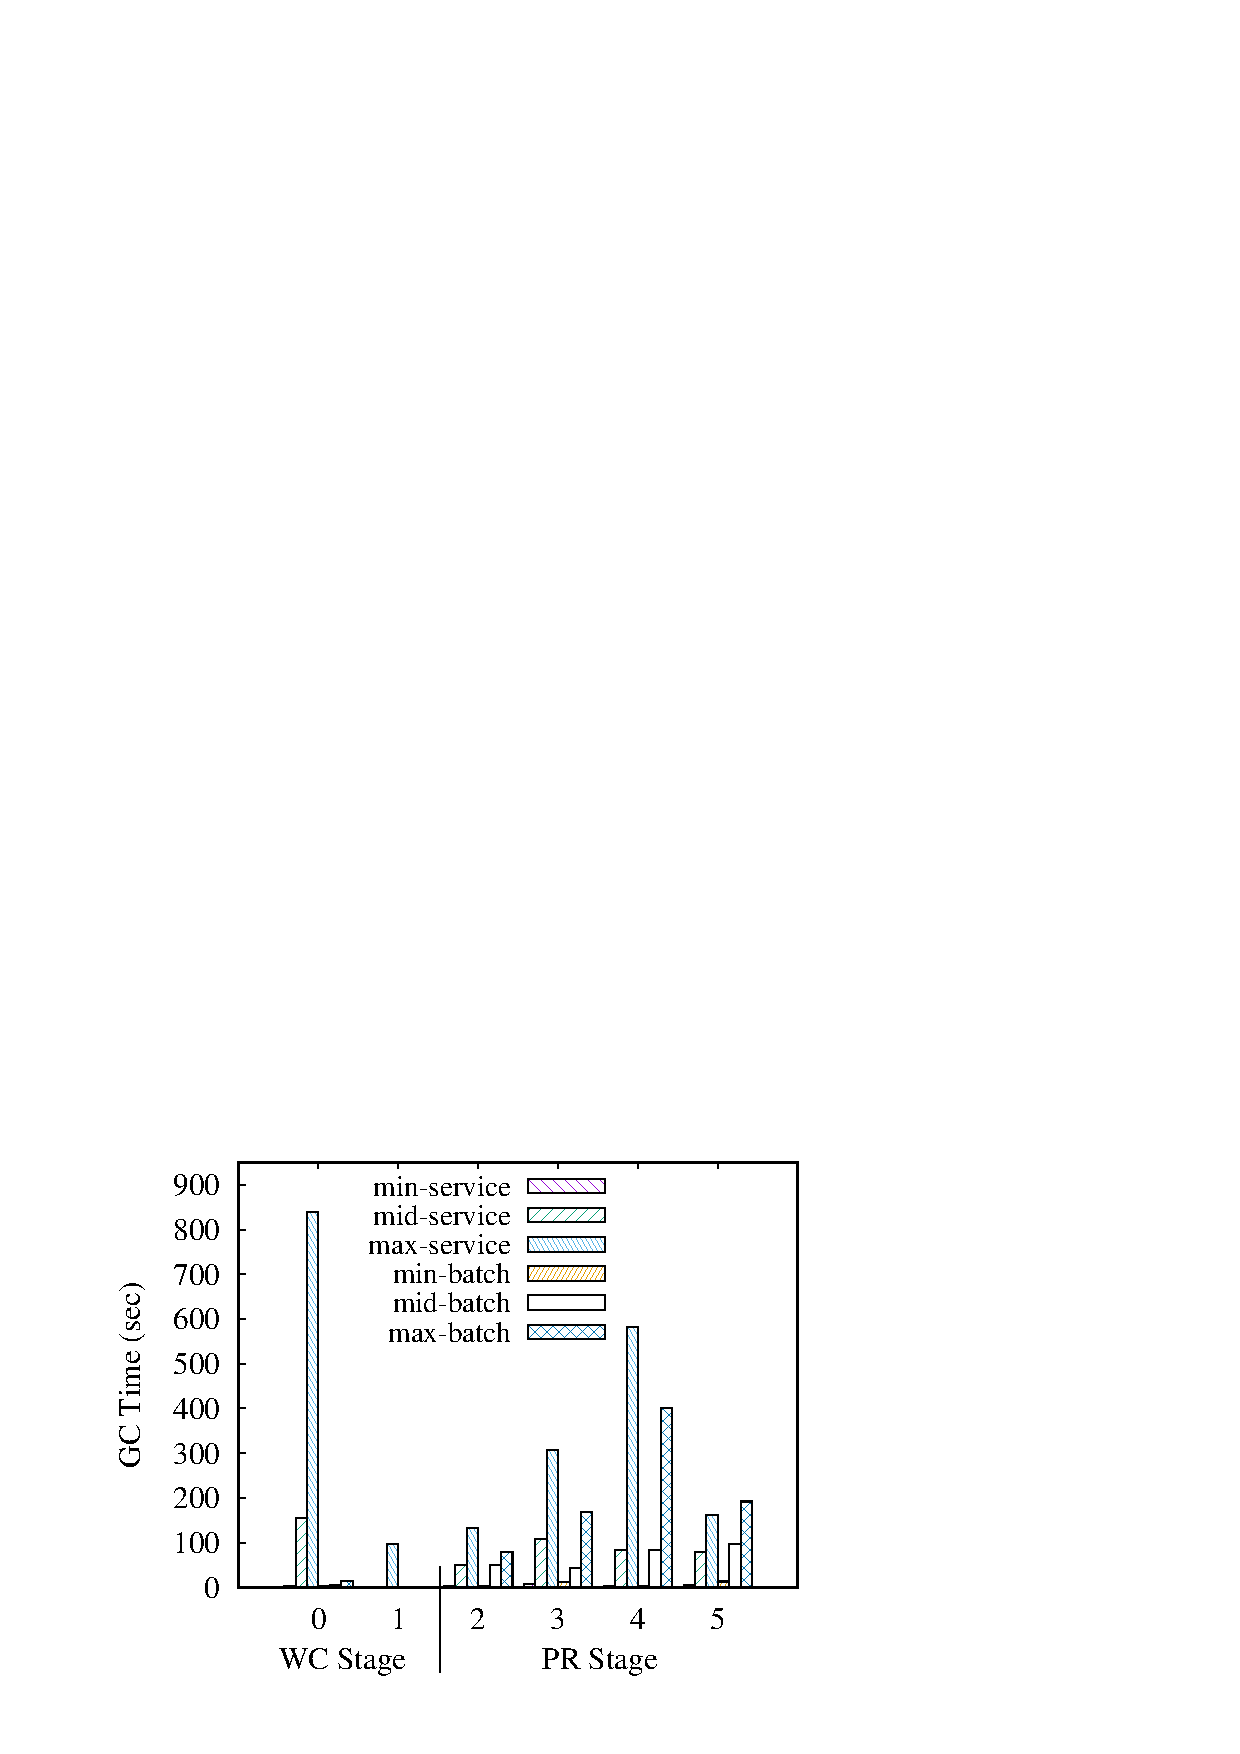
\includegraphics[width=0.231\textwidth]{motivation-gc.pdf}}
\label{fig:wc-result}
\vspace{-2mm}
\caption{The Impact of Memory Pressure}
\vspace{-2mm}
\end{figure}
\end{comment}

%Some applications, such as PR in our observation, they cache intermediate data in memory and iteratively computes the result; one iteration means a stage in Spark. Because the caching data is alive as long as the job, memory space becomes not enough for computation, which means the memory pressure is heavy in PR. However, compare with the PR, WC is another type of task, in which contains only some simple operations, just two stages and very small intermediate shuffle data--though the input data is larger than PR. Furthermore, both the execution time and garbage collection time are low in WC, and the memory pressure is much lighter than PR. The result of PR in batch processing verifies memory pressure and heavy garbage collection (exec-batch and gc-batch in Figure~\ref{fig:memorypressure}). As we can see, the garbage collection time in task accounts for a very great proportion of the execution time.

We observe that PR caches intermediate data in memory and iteratively compute the result. One iteration corresponds to one stage in Spark. Because the caching data is alive as long as the job itself, the memory space becomes gradually less and the task computation will suffer. If this occurs, it indicates the memory pressure caused by PR is heavy. Compare with PR, however, WC only contains some simple operations. WC has only two processing stages and during its execution, a very small amount of intermediate shuffle data are generated (although the input data of WC is larger than that of PR). Furthermore, both the execution time and garbage collection time are low in WC, and the memory pressure is much lighter than PR. The result of PR in the batch mode also verifies its high memory pressure and heavy garbage collection which are the results labelled as exec-batch and gc-batch in Figure~\ref{fig:memorypressure}. As we can see, the garbage collection time accounts for a very large proportion of the execution time.

%PR caches some intermediate data in memory and iteratively computes the result, each iteration means a stage in Spark. The caching data is lived as long as the job, thus available memory space for computation is less which means the memory pressure in PR is heavy. The result of PR in batch processing proves the memory pressure and heavy garbage collection (exec-batch and gc-batch in Figure~\ref{fig:memorypressure}). The garbage collection time in one task has a heavy part in the execution time. However, WC just contains some simple operations and two stages, and the intermediate shuffle data is small although the input data is larger than PR. The memory pressure in WC is light, both the execution time and the garbage collection time is low.

When multiple jobs, such as PR and WC, are submitted to and run by the Spark 
service simultaneously, the jobs are run with a fair scheduler provided by Spark. 
Although WC has much more light memory pressure than PR, all running tasks  
suffer from the heavy memory pressure produced by PR. We find that the execution time 
(exec-service in Figure~\ref{fig:memorypressure} of every task in each stage of PR has little change, except some maximum execution times. This is because 
almost all memory pressure comes from PR and therefore the executions of PR in the service mode and the batch mode show similar trends. However, the execution of WC in the service mode is very different from that in the batch mode. This is because in the service mode, both applications are run simultaneously and therefore WC suffers from the memory pressure produced by PR even if WC is a
light task itself. In the batch mode, since the applications are run one after another. The high memory pressure created by PR will not affect the running of WC.

%If PR and WC are submitted to Spark service, the submitted jobs will run with fair scheduler (provided by Spark). Although PR suffer memory pressure and WC has light memory pressure, all running tasks must suffer the heavy memory pressure produced by PR. We find that the execution time (exec-service in Figure~\ref{fig:memorypressure}) of each task in each stage has a little change in PR except some maximum values. The reason is that almost all memory pressure is coming form PR, running in Spark for service and batch processing is similar. However, WC must suffer the memory pressure produced by PR. The execution time of WC in the first stage has large fluctuation compared to that in batch processing. And we find that the extended time is almost all come from the memory pressure.

In summary, our results implicate that in a system of the service mode, 1) the heavy memory pressure will result in frequent garbage collection, which consumes most of the time and reduce the throughput; 2) the light tasks suffer from heavy memory pressure produced by the heavy tasks; and 3) the heavy tasks obtain the resources later because these resources are occupied chronically by light tasks, and the heavy tasks themselves are the source of memory pressure.

By observing the first stage of PR and WC, we discover that the tasks of PR and WC invoke different function APIs, which determine the impact of each task on memory pressure. If we can identify and classify these tasks by the characteristics of the function APIs, we can suspend the heavy tasks and leave adequate memory space to the light tasks when the memory pressure show up. This can improve the throughput of the service-mode systems and allow all tasks to run with enough memory space and hence light memory pressure.

%Focus on the first stage of PR and WC, we discover that running tasks in PR and WC execute different function APIs. This determines the impact of each task on memory pressure. If we can identify and classify these tasks by the characteristics of function APIs implemented, while the memory pressure comes, we can suspend the heavy tasks and leave enough memory space for the light tasks. This will ensure the throughput of the system for service, and allow all tasks to run with enough memory space and without heavy memory pressure. 

%From the evaluation, we can find that when system is for service, 1) the heavy memory pressure will result in frequent garbage collection which consume most time to cut the throughput. 2) tasks with light memory pressure must suffer the heavy memory pressure produced by others. 3) tasks with heavy memory pressure will get resources later because these resources are occupied longer by these tasks with light memory pressure, and the source of memory pressure is themselves. If we can classify these tasks, when the memory pressure comes, we can stop these tasks which result in heavy memory pressure and remain enough memory space for these tasks which result in light memory pressure. It will ensure the throughput of system for service, and all tasks can run with enough memory space and without heavy memory pressure.  

%While 33\% space are cached data objects that occupy the space with long lifetime, garbage collection will not reclaim these space. We get the cost time and reclaimed space of garbage collection in Figure~\ref{fig:memorypressure}. First, the garbage collections are very frequent and the throughput of job is only 35.7\%. This proves that memory pressure is heavy in the system. Second, the cost of each garbage collection is expensive (GC Time is high in the figure). Some garbage collections which are called full GC will stop the world to mark and clean all the heap. Full GC occurs frequently because the number of lived data objects in memory is too large, it cost more time to mark the lived data objects. Too much lived data objects means less space reclaimed in each garbage collection. Thus, when less space is reclaimed (Reclaimed Space is low in the figure), more time will the garbage collection cost. The worst case is that, frequent garbage collections and less reclaimed space will hinder the performance into the vicious circle.

%Multi-tenant service is provided with the same configurations, we use WordCount, another benchmark in Spark, to balance the execution of PageRank. The dataset of WordCount is produced by HiBench~\cite{www:hibench} and the size is 50GB. The memory usage and garbage collection are the same as the batch processing. %We then consider the completion time with fair scheduler as shown in Figure~\ref{fig:memorypressure2}.
%WC has no cached data, thus memory pressure in WC is lighter and the execution time of WC can be less. However, at first, executors will be lost when jobs are submitted without any configurations tuning. The heavy memory pressure influences the output of disk and network which result in the loss of heartbeat of executors. Second, after the tuning of shuffle configurations, the throughput of WC decreases to 20\%. These tasks without producing much memory pressure must suffer the serious memory pressure from other tenants. %On the other side, PR can also benefit from WC because there are less memory pressure compared to processing batch.

\begin{comment}
\begin{figure}[!t]
\centering
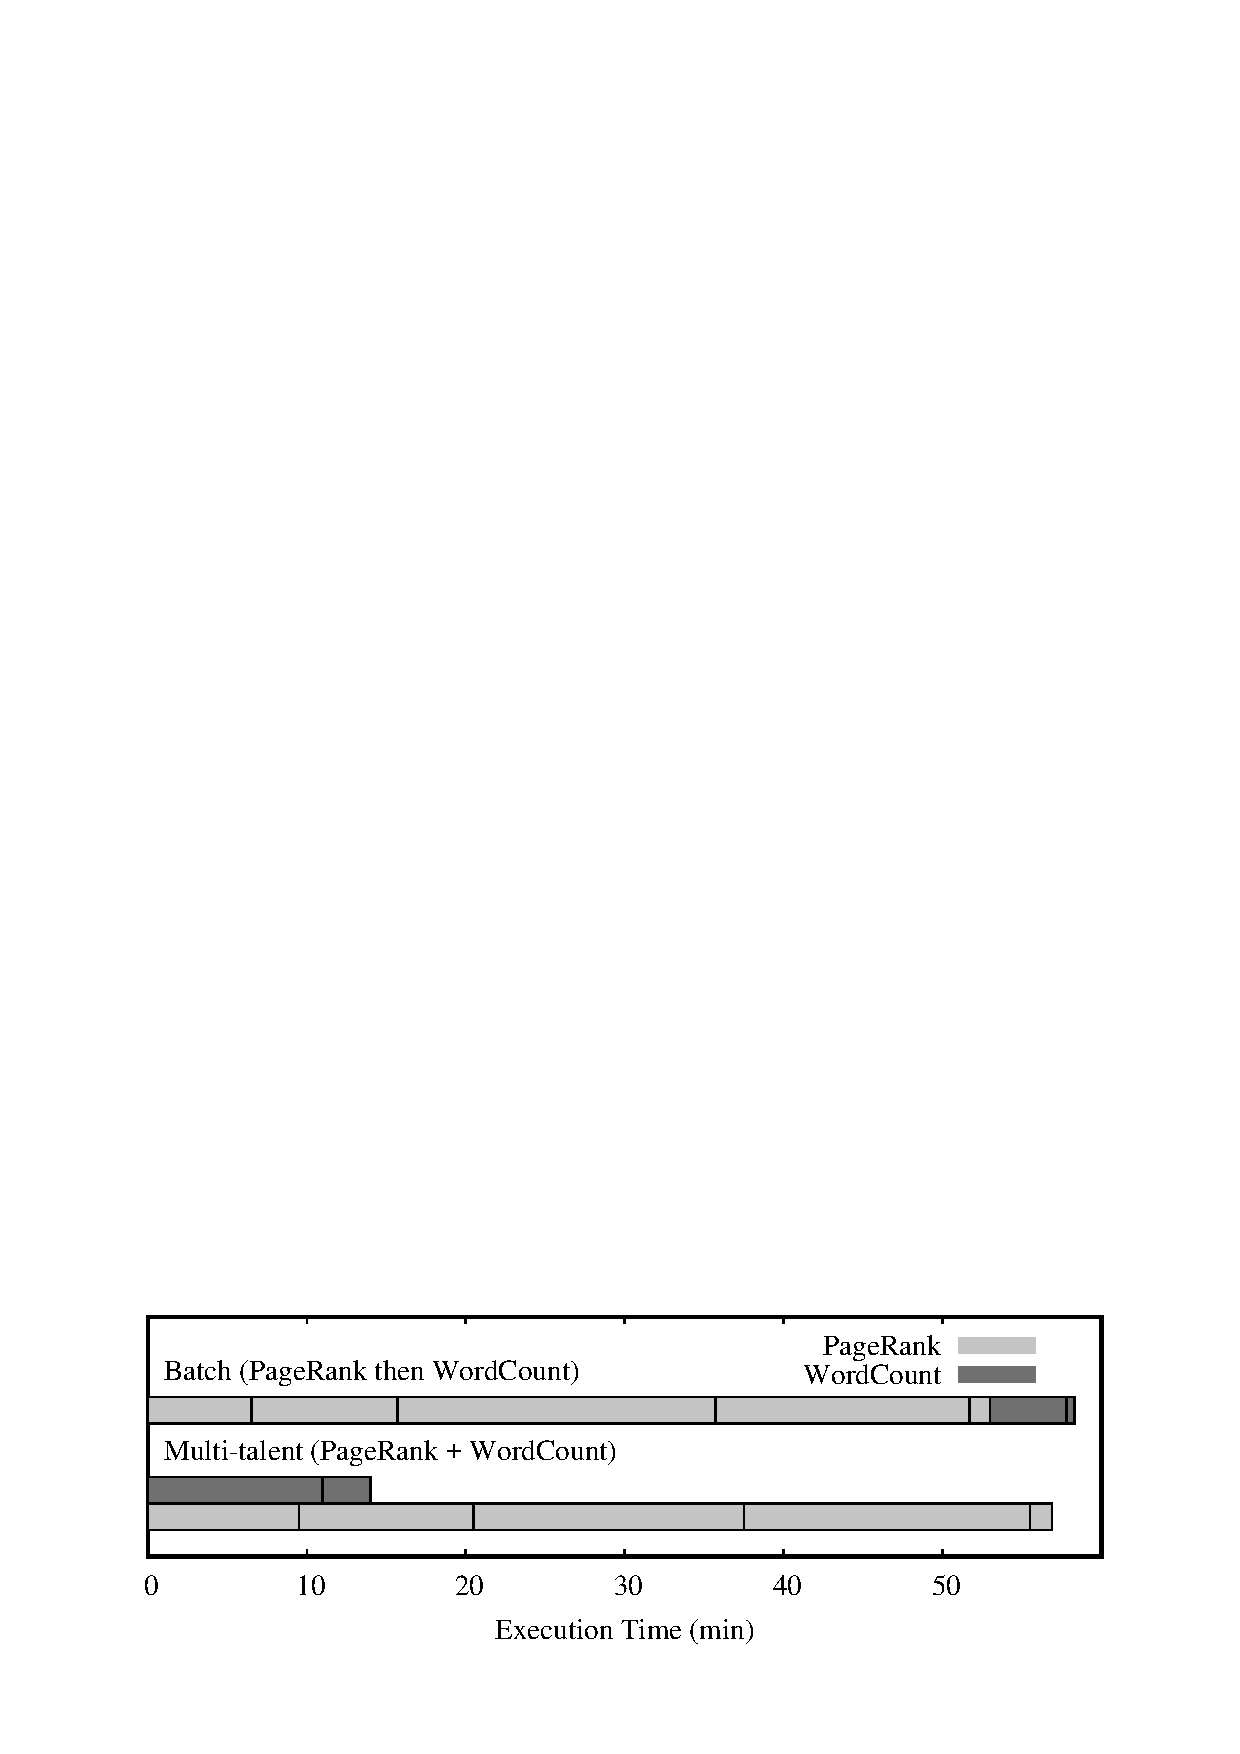
\includegraphics[width=0.45\textwidth]{memorypressure2.pdf}
\caption{Processing Batch and Mutli-tenant}
\label{fig:memorypressure2}
\end{figure}
\end{comment}

%No matter in batch processing or multi-tenant, different tasks can result in different memory pressure. Heavy memory pressure will lengthen the execution time of most tasks and decrease the throughout of jobs. The impact of memory pressure are more complex in multi-tenant in particular. Tasks with heavy memory pressure may benefit from these tasks with light memory pressure. But these tasks with light memory pressure must tolerate the memory pressure from other tasks.

%Although the framework provides several function APIs, these APIs both process the input data as key-value pairs: (key, value). All APIs process key-value pairs according to the key and user-defined functions. Some function APIs like \textit{map} just change the value; some function APIs like \textit{groupByKey} regroup values which have the same key; another function APIs like \textit{reduceByKey} aggregate values by the key. Thus, the result size of value is much different in different function APIs. For example, when one two-tuples is processed, existed key can result in the increase of value in \textit{groupByKey} but non variation in \textit{reduceByKey}. What's more, although different task implements the same function API, the result size in memory may be different because of the processing data type. Through the features of function APIs, we can classify the memory usage rate of function APIs to four type: \textbf{Constant}, \textbf{Sub-linear}, \textbf{Linear} and \textbf{Super-Linear}. After coarse-grained dividing the tasks implement function APIs to different types, when the memory pressure comes, these tasks lead to more memory pressure is clear.  

\section{Related Work}

%Related works of this paper include these aspects:

% 机器学习在GPU性能分析上的应用实例。完全用机器学习预测和分析IPDPS16、HPCA15;
% 在AM模型上使用机器学习ICPE15。
% 另外需要提一下ML在特征工程上的重要性工作。

%Machine Learning in GPU performance analysis~\cite{nguyen:yak}. 

%Feature engineering in ML is also the basis of our work.

% 传统的性能分析模型的应用实例,通用模型方面,GPU架构HPCA11、应用本身的性能指标DATE16、应用的优化措施分析PPoPP12; 
% 专用模型方面,稀疏矩阵CC15、程序并行性ICPPW12、程序中判断条件的性能CCPE13
% 等。

%Analytical Model in GPU performance analysis is built on general cases or proprietary cases.
%General cases:
%architecture of GPU system. For example, work 1; work 2.
%optimization of GPU application. For example, work 3.
%runtime metrics of GPU applications. For example, work 4.
%Proprietary cases:
%SPMV; Parallelism; Conditions in instructions.

There is plenty of work on performance evaluation of GPU application, including traditional performance analysis models(AM) and machine learning-based approaches(ML). AM can be classified into general models and specific models. General models are generally applicable to any GPU program or kernel, and provide a comprehensive assessments, while specific models are for specific GPU programs or provide assessment for part of GPU architecture.

Zhang and Owens~\cite{Zhang2011A} propose a quantitative performance analysis model from the perspective of GPU architecture, in which they modele the execution time spent on the instruction pipeline, shared memory, and global memory, to find performance bottleneck of GPU application. Sim et al.~\cite{Sim2012A} present an analysis model from the perspective of application optimization methods. They classify the methods into four aspects and put forward four potential benefit metrics: B$_{itilp}$, B$_{memlp}$, B$_{fp}$, B$_{serial}$, to guide application performance optimization. Bombieri et al.~\cite{Bombieri2016A} propose a fine-grained performance model based on the performance metrics of GPU application, such as synchronization, thread divergence, load balancing, L1/L2, shared memory efficiency. The model rely on micro-benchmarks and several optimization criteria to estimate the potential performance of the application.

As for specific models, some researches are on specific GPU application. Guo and Wang~\cite{Guo2015Accurate} propose an analytical approach to predict the kernel execution time of sparse matrix-vector multiplications. Su et al.~\cite{Su2015An} present a performance analysis model for 3D stencil calculations based on the data transfer at different stages of the GPU memory hierarchy. Some researches focuses on one kind of GPU applications, for example, an analytic model that focuses on memory-bound applications is discribed in~\cite{Ma2012A}. Models for only one aspect of GPU also exist. Konstantinidis and Cotronis~\cite{Konstantinidis2016A} describe a performance evaluation for measuring the memory bandwidth of fast on-chip memories of GPU.

Traditional performance analysis models, although accurate, often require a detailed understanding of the hardware architecture, and they often rely on simulators or profiling tools to collect information, which is time-consuming. More and more researches use machine learning approaches to carry out performance evaluation.

Wu et al.~\cite{Wu2015GPGPU} describe a GPU performance and power estimation model, using machine learning method to explore the design space for different hardware configurations, and use the performance values in one configuration to predict performance and power in other configurations. Madougou et al.~\cite{Madougou2016A} present a statistical method for performance analysis based on hardware performance counters, using random forest algorithms combined with PCA (principal component analysis) and regression methods to identify performance bottlenecks and predict performance of GPU applications.

Performance evaluation based on machine learning is simple and easy to use, but its accuracy can not be guaranteed since it strongly depends on the training data sets, and feature selection is also very important. Didona et al.~\cite{Didona2015Enhancing} combine traditional analysis model with machine learning method, taking AM as an individual, and compares it with ML-based modeling to improve the robustness of performance prediction. But this method is not for GPU applications.

In our work, we combine machine learning approach with analysis model to conduct the performance evaluation. The process is divided into two stages. In the first stage, machine learning method is used to train and obtain the most influential features on GPU application execution time, and the features are sorted based on the degree of the influence. In the second stage we use the analysis model to analyze these features and identify the performance bottleneck.


\section{Background}

\subsection{Features in ML}

% 特征工程是机器学习应用中重要的两个模块之一,特征用来评价一条记录的某个方面,特征的好坏决定了模型的准确性。
% 机器学习对特征的要求是各个特征之间的依赖性很小,尽量相互独立,能够反映数据的特点。例如,GPU应用的一条监控数据,包括三个特征:Kernal函数的程序长度Code_Line,编译后的Kernal函数指令条数Instruction_Line,SM配置的Block的维度Block_X,Code_Line和Instruction_Line有明显的决定关系,两者关联度很高,在一般情况下Code_Line和Instruction_Line成线性关系,作为两个特征并不合适,而Block_X和Instruction_Line之间没有直接关系,可以作为两个重要特征。

% 在计算要求较高的机器学习应用中,往往需要对特征做降维处理。降维处理是从特征体系中选择最为重要的特征,一般的降维算法有PCA、信息熵决策。决策方法通过信息理论熵计算出最重要的特征,即降维时需要选择的特征。

Features in ML.

\subsection{Decision Model in ML}

% 机器学习的训练模型中有两大类,基于线性拟合的模型(Regression Model),如逻辑回归(Logistics Regression),神经网络(Neural Network),深度学习(Deep Learning)等;基于信息论的决策模型(Decision Model),如决策树(Decision Tree),随机森林(Random Forest)等。
% 机器学习模型的训练本质上是对特征的处理:Regression Model通过多次迭代,更新模型中各项特征的权重矩阵,最终权重矩阵收敛到一个稳定值;Decision Model则通过多次划分,每次选择最优的特征来划分数据集,形成树形模型。

% 在对新的数据做分类预测时,Regression Model直接利用权重矩阵与新数据的特征值矩阵相乘,预测新数据的类别,而Decision Model则按照树形模型依次考虑新数据的每个特征值所属类别。因此,Decision Model更适合于分析预测的过程,而且基于信息论的决策过程同样适用于特征降维,可以保证数据特征选取的科学性。
% 在Decision Model上最基础的实现是Decision Tree,基于信息划分理论实现Decision Tree。在Decision Tree基础上发展的Random Forest则通过多颗树形成森林,然后对结果做综合预测,进一步提高机器学习模型的准确性。

% 在GPU应用的监控数据中,我们需要考虑监控数据的重要性,首先需要做的是将监控的metric转变为Feature,形成一条记录。然后选择机器学习的模型来决定重要的Feature,很明显Decision Model更适合于中间过程的分析。由于机器学习模型极大的方便了用户,屏蔽了非常重要的技术分析细节,准确率往往比传统的数学模型要低。为了保证GPU应用分析的重要性,结合传统的数学分析模型更为重要。所以使用Decision Tree而不是Random Forest,对使用理论模型分析性能的情况更为高效。

Decision model in ML.

\subsection{GPU}

GPU architecture.
\section{Decision Tree}

% (全文指标和监控数据统一用metric表示,特征用feature表示,但是二者可以等同为同一个意思。在ML中称为feature,在AM中称为metric)

% 各种监控工具以及各种监控的数据,产生了许多指标数据,让GPU的性能分析变得异常复杂。Decision Tree可以利用信息理论筛选出最重要的指标集,更方便、快速地利用GPU架构的理论知识发现性能瓶颈并给出优化方案。

\subsection{Features and Hypothesis Space}

% 建立决策树模型的第一步需要形成特征体系。一个GPU microBenchmark可以形成一条记录,并且可以产生多种监控数据。
% 这些监控数据可以分为两类:一类与用户提交应用时指定的数据集、硬件固有属性等有关,例如输入数据集的大小,Global memory的带宽等;另一类是事实上反应了当前GPU架构和GPU应用架构下的运行特征,例如Global Memory的load/store数、L1 cache的命中率、Instruction的并行度等。
% 这两类数据都决定了一个GPU microBenchmark的运行结果,并且反映了一次运行的性能信息。
% 所以我们可以直接利用监控的metric作为一条记录的Feature。也就是说,一个metric就是一个feature。同时我们将用户指定或者硬件固有属性等不形容运行状态的Feature称为Static Feature(SF),而将形容运行状态Feature称为Runtime Feature(RF)。

% 在ML的特征工程中,除了监控可得的特征,还可以通过特征之间的非线性计算方法得到新的特征。例如,访问L1 cache的次数和访问Global memory的次数是两个特征,通过除法可以得到Global Memory的访问命中率,Global memory的访问命中率也可以作为一个新的特征。
% 传统的数学分析模型也提供了诸多的性能指标计算方法,这些都可以作为新的特征添加到特征体系中。我们将这种特征称为Assistant Feature(AF)。SF、RF和AF共同组成了GPU性能分析的特征体系。常用的特征值/指标值的含义及特征类型如表~\ref{table:metrics}所示。

Common examples of metrics (or features) used in this paper are shown in Table~\ref{table:metrics}.

\begin{table}[!t]
\small
%\lefting
\caption{Common Examples of Metrics/Features in this paper} 
\begin{tabular}{ l | l | l }
\hline
\textbf{Name} & \textbf{Metric Meaning} & \textbf{Type} \\
\hline
\textit{Input\_size} & size of input dataset & SF\\
\hline
\textit{TLP} & the thread level parallelism & RF \\
 \hline
\textit{ILP} & the instruction level parallelism & RF \\
\hline
\textit{SFU\_width} & width of special function units per SM & RF \\
\hline
\textit{Cache\_hit} & cache hit latency & RF \\
\hline
\textit{Sync\_over} & the overhead of waiting synchronization & AF \\
\hline
\end{tabular}
%\vspace{-4mm}
\label{table:metrics}
\end{table}

% 不可忽略的是在诸多的监控数据中存在具有一定关联性的特征值,因为往往一个性能瓶颈会影响多项类似的指标异常。例如数据放置不均衡,会导致L1 cache的load次数增加,同时必然导致Global memory的load次数增加,这两个特征值之间有一定的关联性。
% 这类关联特征往往一起影响GPU应用的运行状态,但是最终指向同一个关键因素,我们将这类特征/指标归结为一个特征集/指标集。在决策树模型中,每次决策选择当前最重要的特征,多次决策就可以得到一个特征集。在ML中,特征集之间的关联性往往会影响模型的准确性。但是我们后续基于特征集进行理论分析,不仅可以避免特征之间的关联性带来的模型的不准确性,还可以利用这个关联性定位性能瓶颈。

% 根据特征体系,我们可以得到用于决策的假设空间。假设空间可以确定特征值的有效性,决定是否能够建立决策树模型。要建立假设空间,必须考虑到每次监控的特征值不可能完全相同。因此,我们需要通过缩小监控值的精度,限定特征值的范围来建立假设空间。
% 分析GPU性能的Decision Tree的一个可能的假设空间如图~\ref{fig:hs}所示。假设空间的每一层都有一个关键的特征作为划分依据,根据特征的可能出现的值划分成多个数据集。

One possible hypothesis space of this paper is shown in Figure~\ref{fig:hs}.

\begin{figure}[!t]
\centering
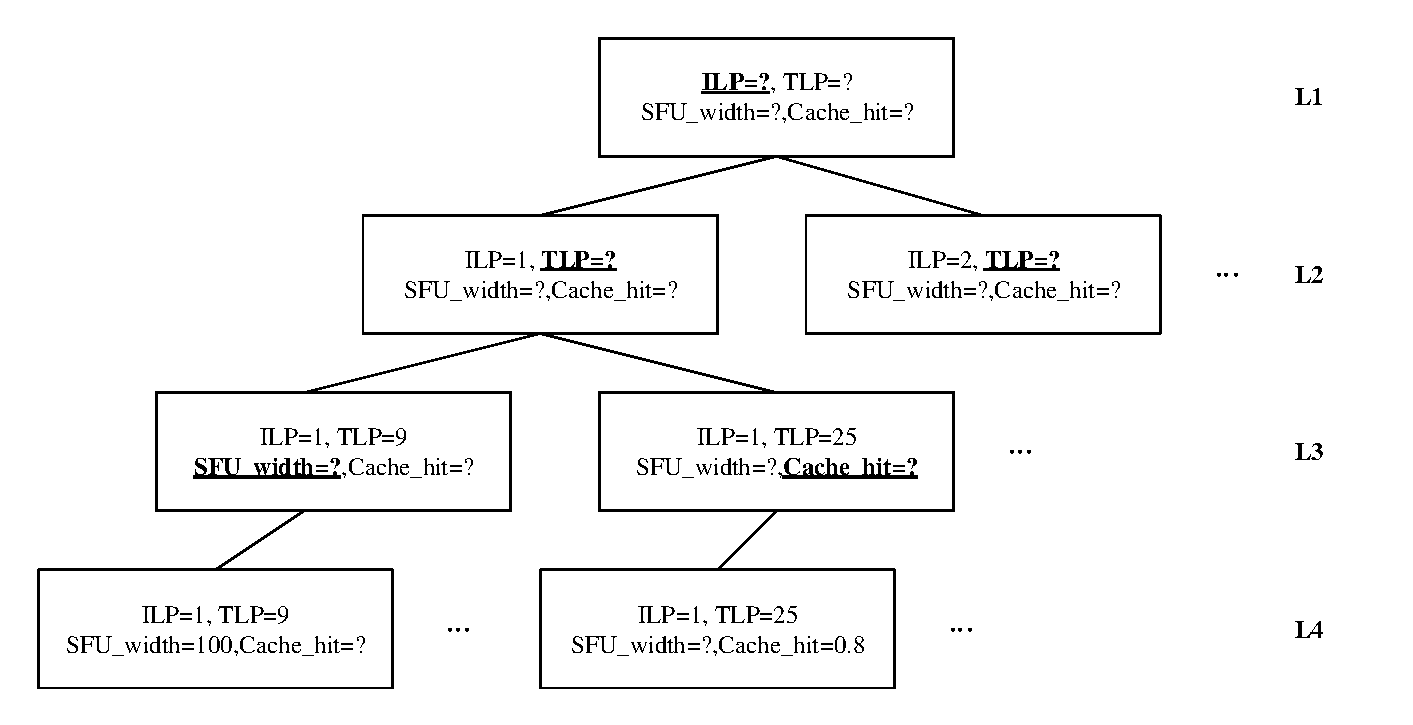
\includegraphics[width=0.5\textwidth]{hypothesisspace.pdf}
%\vspace{-2mm}
\caption{An Example of Hypothesis Space}
%\vspace{-4mm}
\label{fig:hs}
\end{figure}

\subsection{Training Set}

We choose these benchmarks to build the training set:

\begin{itemize}

\item micro-benchmarks

\item Pariol benchmarks.

\item Regal benchmarks.

\end{itemize}

\subsection{Decision Tree}
\label{subsec:decisiontree}

Decision Tree.


\section{Design of MURS}
\label{sec:desgin}

Memory pressure essentially describes the usage of heap in managed languages. We first compute the heavy tasks which may have linear or super-linear model, or have large input dataset. The fundamental scheduling mechanism is suspending these heavy tasks as memory pressure occurs, and then resuming the suspended task when memory pressure recedes or light task completes.

%\subsection{Memory management}

%// 这一段的目的不够明确

%Although the memory usage rate describes the memory usage features about different tasks, we should also separate the memory management of the data processing system itself and JVM. Because the data processing systems always take some measures to avoid the out of memory error by spilling data to disk which based on the memory management themselves. When the spill occurs, the memory may suffer pressures although we stop tasks.

%Most data processing systems split the allocated memory to cache memory and execution memory. The cache memory is only used to store data with long lifetime. While execution memory is only used for temporary or middle data, such as shuffle result that will be write to disk. Cache memory and execution memory can be managed uniformly. What's more, these execution memory are allocated to each task independently. These make up the memory management of data processing system and also decide the memory usage rate of one task based the function API. When considering about the memory pressure, it's conflict to consider the memory management of data processing system. Because after one task is completed, the allocated execution memory will be reclaimed but the data objects are also in JVM heap. On another hand, some tasks will not only use the execution memory but also cache memory. Thus, in order to measure the memory pressure, we just consider the usage of JVM heap but not the memory management of data processing system.

%In the memory management of JVM, the heap space is split to young generation, old generation and other generations. The pinch of young generation leads to \textit{Minor GC}. Minor GC will move the lived data objects from young generation to old generation. The pinch of old generation leads to Full GC. If most long lifetime data objects remain in the old generation, frequent full gc will occur and lead to bad performance. Some garbage collection algorithms are working only in young generation or old generation, and some can works on both generations. In any case, the garbage collection is triggered when the used space of heap get the threshold.

Firstly, we define the memory pressure as follows: when the proportion of used heap has reached the threshold value. The threshold is set according to the trigger of garbage collection. In addition, we set two thresholds here. The first threshold, called as yellow value, is used to indicate the memory pressure. When the percentage of long lived data objects in the heap meets the yellow value, it means frequent full GC will occur. Full GC means that the garbage collector will clean all the heap, and it is usually expensive. Another threshold value, called as red value, is used to avoid spilling. The red value shows the pressure under which the out-of-memory error will occur or some data will be spilled to disk. The default values of yellow and red are 0.4 and 0.8, based on our evaluation. It is proposed that, if the memory pressure is heavy, we should reduce the value.

With the yellow and red value, an accurate percentage of long lived data objects in the heap actually determines the efficiency of threshold. As JVM splits the heap to young generation and old generation, minor GC cleans the young generation and moves alive data objects to the old generation. Thus the percentage of heap usage after a minor GC describes the lived data objects in the heap. After each full GC, dead data objects in old generation will also be reclaimed, we revise the percentage of long lived data objects in the heap according to the current percentage of heap usage.

%With the yellow value and red value, the percentage of data objects with long lifetime in the heap are actually important. As we know, garbage collection algorithm is based on mark-clean; thus, long-lived data objects in the heap will lead to expensive marking and cleaning costs. What’s more, long-lived data objects directly result in frequent full garbage collection. In order to get the percent of long lifetime data objects in heap, we set it to the size after a minor GC, which just cleans parts of the heap quickly. These data objects are lived in the heap, and most will also be lived along with the tasks.  

%Although the scheduler wishes to reclaim as many data objects as possible, the space reclaimed the last time will have an error with the expected reclaimed space. The error actually means the space occupied by these data objects was stored in an old generation and reclaimed before the task completed. We count the error and consider it in the last computation. Because tasks themselves work with the iterator, the produced data objects have steady regulars.

\IncMargin{0.4em}
\SetAlFnt{\small}
\begin{algorithm}[!t]
%\DontPrintSemicolon

\SetKwInOut{Input}{Input}\SetKwInOut{Output}{Output}
\SetKwProg{Fn}{Function}{}{end}
\SetKwFunction{CST}{ComputeSuspendTasks}
\SetKwFunction{CS}{ComputeSpill}
\SetKwData{F}{\small{final}}

\Input{Array of running tasks $R$\;}
\Output{Array of suspended tasks $S$\;}
get the Memory Usage Sampler $Sampler$\;
get the Memory Manger $SM$ of System\;
get the Memory Manger $JM$ of JVM\;
get the queue including suspended tasks $SQ$\;
\lIf{Usage of $JM$ is lower than the yellow value}{return}
\lElseIf{Usage of $JM$ is lower than the red value}{\CS}
\lElseIf{$SQ$ is not empty}{return}
\lElse{\CST}

\BlankLine
\Fn{\CST}{
  $freeMemory \leftarrow JM.freeMemory$\;
  $consumption[] \leftarrow SM.tasksMemoryConsumption$\;
  $rate[] \leftarrow Sampler.getMemoryUsageRate$\;
  $percent[] \leftarrow Sampler.getCompletePercent$\;
  $S \leftarrow R$\;
  \While{$freeMemory > 0$}{
    $minRateTaskId \leftarrow reate[].min$\;   
    \lIf{\CS}{reduce the running cores and return}
    $memoryNecessary \leftarrow comsumption[taskId] * (1-percent[taskId])$\;
    $freeMemory -= memoryNecessary$ \;
    $S$ remove minRateTaskId \;
    push minRateTaskId to $SQ$\;
    $rate[]$ remove minRateTaskId \;
  }
  \KwRet{$S$}
}
\BlankLine
\Fn{\CS}{
  $taskId \leftarrow$ task Id \;
  $totalMemory \leftarrow JM.totalMemory$ \;
  \lIf{$comsumption[taskId] > totalMemory / R.length$}{\KwRet{True}}
  \Else{
      $memoryNecessary \leftarrow comsumption[taskId] / percent[taskId]$\;
      \lIf{$memoryNecessary > totalMemory / R.length$}{\KwRet{True}}
      \lElse{\KwRet{False}}
      }
}
\caption{Scheduling mechanism on JVM}
%\vspace{-4mm}  
\label{code:scheduler}
\end{algorithm}

These indicators of memory pressure are the infrastructure of the memory usage rate based scheduler. The scheduler is designed in Algorithm~\ref{code:scheduler}. The input is the current running tasks and the output is the proposed suspended tasks. Some basic managers should be accessible to record the indicators of memory pressure. We design a \textit{Sampler} to record the real-time metrics of current running tasks. Sampler runs seasonally to update the metrics of each task and compute the current memory usage rate, such as the size of input dataset, the number of processed records, and the size of result data.

If the memory pressure is light, or the system already has suspended tasks, we directly return without propose (lines 4, 6). If the memory pressure has reached the red value, MURS will avoid spilling (line 5). When the memory usage of JVM heap touches the yellow value, we get the memory usage rates of all running tasks from the sampler and other details of current memory (lines 9-12). We take the measures to process current running tasks step by step in the following order: constant, sub-linear, linear, and super-linear. Free memory subtracts the necessary memory of the currently processing task every time. When free memory is not enough for the remaining unprocessed tasks, scheduler will stop processing tasks (lines 14-20). This method is able to distinguish these tasks with sub-linear model but working as heavy tasks if they process larger dataset, or tasks with super-linear model but working as light tasks if they consume less memory space. Processed tasks are removed and the remained tasks will be returned. The returned tasks are heavy tasks and will be set to suspend. In order to avoid potential starvation, suspended tasks are pushed to a queue (line 21). FIFO algorithm allows us to resume the first suspended task to avoid starvation. 

MURS suspends the proposed heavy tasks to prevent memory pressure increasing at a high rate of speed. Note that if all running tasks are heavy tasks, MURS still schedule tasks with the same algorithm. It always chooses these tasks have relatively small memory usage rate in total tasks. 

Function \textit{ComputeSpill} is designed to avoid spilling. As the running tasks share the JVM heap together, the maximally allocated space for each task is ensured to less than $1/N$ while $N$ is the number of running threads. When the consumption exceeds the maximal space, the spill or out-of-memory error will occur. Running tasks that satisfy the \textit{ComputeSpill} (lines 27, 30) are also suspended to decrease the parallelism in order to acquire enough memory space after memory pressure goes away.   

When a running task completes, we resume a suspended task popped from the queue accordingly. After the memory pressure recedes, meaning the usage of JVM heap is below the yellow value after a full GC, the remaining suspended tasks will also be removed. However, one completed task only resumes one suspended task and the memory usage below yellow value will remove all suspended tasks.
\section{Evaluation}

\subsection{Configuration}

We use four nodes as workers and one node as the master in the experiments. Each node has two eight-core Xeon-2670 CPUs and 64GB memory. The file system is mount on one SAS disk, running RedHat Enterprise Linux 5 (kernel 2.6.18). The JDK version is 1.7.0 for Spark 1.6 and Spark Job Server 0.6.2. We count not only the execution time of each application, but also the details of runtime situations.
%\section{Related Work}

%Related works of this paper include these aspects:

% 机器学习在GPU性能分析上的应用实例。完全用机器学习预测和分析IPDPS16、HPCA15;
% 在AM模型上使用机器学习ICPE15。
% 另外需要提一下ML在特征工程上的重要性工作。

%Machine Learning in GPU performance analysis~\cite{nguyen:yak}. 

%Feature engineering in ML is also the basis of our work.

% 传统的性能分析模型的应用实例,通用模型方面,GPU架构HPCA11、应用本身的性能指标DATE16、应用的优化措施分析PPoPP12; 
% 专用模型方面,稀疏矩阵CC15、程序并行性ICPPW12、程序中判断条件的性能CCPE13
% 等。

%Analytical Model in GPU performance analysis is built on general cases or proprietary cases.
%General cases:
%architecture of GPU system. For example, work 1; work 2.
%optimization of GPU application. For example, work 3.
%runtime metrics of GPU applications. For example, work 4.
%Proprietary cases:
%SPMV; Parallelism; Conditions in instructions.

There is plenty of work on performance evaluation of GPU application, including traditional performance analysis models(AM) and machine learning-based approaches(ML). AM can be classified into general models and specific models. General models are generally applicable to any GPU program or kernel, and provide a comprehensive assessments, while specific models are for specific GPU programs or provide assessment for part of GPU architecture.

Zhang and Owens~\cite{Zhang2011A} propose a quantitative performance analysis model from the perspective of GPU architecture, in which they modele the execution time spent on the instruction pipeline, shared memory, and global memory, to find performance bottleneck of GPU application. Sim et al.~\cite{Sim2012A} present an analysis model from the perspective of application optimization methods. They classify the methods into four aspects and put forward four potential benefit metrics: B$_{itilp}$, B$_{memlp}$, B$_{fp}$, B$_{serial}$, to guide application performance optimization. Bombieri et al.~\cite{Bombieri2016A} propose a fine-grained performance model based on the performance metrics of GPU application, such as synchronization, thread divergence, load balancing, L1/L2, shared memory efficiency. The model rely on micro-benchmarks and several optimization criteria to estimate the potential performance of the application.

As for specific models, some researches are on specific GPU application. Guo and Wang~\cite{Guo2015Accurate} propose an analytical approach to predict the kernel execution time of sparse matrix-vector multiplications. Su et al.~\cite{Su2015An} present a performance analysis model for 3D stencil calculations based on the data transfer at different stages of the GPU memory hierarchy. Some researches focuses on one kind of GPU applications, for example, an analytic model that focuses on memory-bound applications is discribed in~\cite{Ma2012A}. Models for only one aspect of GPU also exist. Konstantinidis and Cotronis~\cite{Konstantinidis2016A} describe a performance evaluation for measuring the memory bandwidth of fast on-chip memories of GPU.

Traditional performance analysis models, although accurate, often require a detailed understanding of the hardware architecture, and they often rely on simulators or profiling tools to collect information, which is time-consuming. More and more researches use machine learning approaches to carry out performance evaluation.

Wu et al.~\cite{Wu2015GPGPU} describe a GPU performance and power estimation model, using machine learning method to explore the design space for different hardware configurations, and use the performance values in one configuration to predict performance and power in other configurations. Madougou et al.~\cite{Madougou2016A} present a statistical method for performance analysis based on hardware performance counters, using random forest algorithms combined with PCA (principal component analysis) and regression methods to identify performance bottlenecks and predict performance of GPU applications.

Performance evaluation based on machine learning is simple and easy to use, but its accuracy can not be guaranteed since it strongly depends on the training data sets, and feature selection is also very important. Didona et al.~\cite{Didona2015Enhancing} combine traditional analysis model with machine learning method, taking AM as an individual, and compares it with ML-based modeling to improve the robustness of performance prediction. But this method is not for GPU applications.

In our work, we combine machine learning approach with analysis model to conduct the performance evaluation. The process is divided into two stages. In the first stage, machine learning method is used to train and obtain the most influential features on GPU application execution time, and the features are sorted based on the degree of the influence. In the second stage we use the analysis model to analyze these features and identify the performance bottleneck.


\section{Conclusion}

In order to mitigate the memory pressure in current data processing systems for service, this paper analyzes the memory usage characters of variety function APIs provided by these systems and build three coarse grained models to classify them, then proposes memory usage rate as a uniform criterion to mark the influence of one task on memory pressure. The memory usage rate based scheduler called MURS can suspend these tasks resulting in heave memory pressure, and speed up these tasks with light memory pressure. MURS can be implemented in most data processing systems.

%\section{Introduction}
% no \IEEEPARstart
%This demo file is intended to serve as a ``starter file''
%for IEEE conference papers produced under \LaTeX\ using
%IEEEtran.cls version 1.7 and later.

%All manuscripts must be in English. These guidelines include complete descriptions of the fonts, spacing, and related information for producing your proceedings manuscripts. Please follow them and if you have any questions, direct them to the production editor in charge of your proceedings at Conference Publishing Services (CPS): Phone +1 (714) 821-8380 or Fax +1 (714) 761-1784.
% You must have at least 2 lines in the paragraph with the drop letter
% (should never be an issue)

%\subsection{Subsection Heading Here}
%Subsection text here.


%\subsubsection{Subsubsection Heading Here}
%Subsubsection text here.

%\section{Type style and Fonts}
%Wherever Times is specified, Times Roman or Times New Roman may be used. If neither is available on your system, please use the font closest in appearance to Times. Avoid using bit-mapped fonts if possible. True-Type 1 or Open Type fonts are preferred. Please embed symbol fonts, as well, for math, etc.


% An example of a floating figure using the graphicx package.
% Note that \label must occur AFTER (or within) \caption.
% For figures, \caption should occur after the \includegraphics.
% Note that IEEEtran v1.7 and later has special internal code that
% is designed to preserve the operation of \label within \caption
% even when the captionsoff option is in effect. However, because
% of issues like this, it may be the safest practice to put all your
% \label just after \caption rather than within \caption{}.
%
% Reminder: the "draftcls" or "draftclsnofoot", not "draft", class
% option should be used if it is desired that the figures are to be
% displayed while in draft mode.
%
%\begin{figure}[!t]
%\centering
%\includegraphics[width=2.5in]{myfigure}
% where an .eps filename suffix will be assumed under latex, 
% and a .pdf suffix will be assumed for pdflatex; or what has been declared
% via \DeclareGraphicsExtensions.
%\caption{Simulation Results}
%\label{fig_sim}
%\end{figure}

% Note that IEEE typically puts floats only at the top, even when this
% results in a large percentage of a column being occupied by floats.


% An example of a double column floating figure using two subfigures.
% (The subfig.sty package must be loaded for this to work.)
% The subfigure \label commands are set within each subfloat command, the
% \label for the overall figure must come after \caption.
% \hfil must be used as a separator to get equal spacing.
% The subfigure.sty package works much the same way, except \subfigure is
% used instead of \subfloat.
%
%\begin{figure*}[!t]
%\centerline{\subfloat[Case I]\includegraphics[width=2.5in]{subfigcase1}%
%\label{fig_first_case}}
%\hfil
%\subfloat[Case II]{\includegraphics[width=2.5in]{subfigcase2}%
%\label{fig_second_case}}}
%\caption{Simulation results}
%\label{fig_sim}
%\end{figure*}
%
% Note that often IEEE papers with subfigures do not employ subfigure
% captions (using the optional argument to \subfloat), but instead will
% reference/describe all of them (a), (b), etc., within the main caption.


% An example of a floating table. Note that, for IEEE style tables, the 
% \caption command should come BEFORE the table. Table text will default to
% \footnotesize as IEEE normally uses this smaller font for tables.
% The \label must come after \caption as always.
%
%\begin{table}[!t]
%% increase table row spacing, adjust to taste
%\renewcommand{\arraystretch}{1.3}
% if using array.sty, it might be a good idea to tweak the value of
% \extrarowheight as needed to properly center the text within the cells
%\caption{An Example of a Table}
%\label{table_example}
%\centering
%% Some packages, such as MDW tools, offer better commands for making tables
%% than the plain LaTeX2e tabular which is used here.
%\begin{tabular}{|c||c|}
%\hline
%One & Two\\
%\hline
%Three & Four\\
%\hline
%\end{tabular}
%\end{table}


% Note that IEEE does not put floats in the very first column - or typically
% anywhere on the first page for that matter. Also, in-text middle ("here")
% positioning is not used. Most IEEE journals/conferences use top floats
% exclusively. Note that, LaTeX2e, unlike IEEE journals/conferences, places
% footnotes above bottom floats. This can be corrected via the \fnbelowfloat
% command of the stfloats package.



%\section{Conclusion}
%The conclusion goes here. this is more of the conclusion

% conference papers do not normally have an appendix


% use section* for acknowledgement
%\section*{Acknowledgment}


%The authors would like to thank somebody and somebody. The work is provided by 


% trigger a \newpage just before the given reference
% number - used to balance the columns on the last page
% adjust value as needed - may need to be readjusted if
% the document is modified later
%\IEEEtriggeratref{8}
% The "triggered" command can be changed if desired:
%\IEEEtriggercmd{\enlargethispage{-5in}}

% references section

% can use a bibliography generated by BibTeX as a .bbl file
% BibTeX documentation can be easily obtained at:
% http://www.ctan.org/tex-archive/biblio/bibtex/contrib/doc/
% The IEEEtran BibTeX style support page is at:
% http://www.michaelshell.org/tex/ieeetran/bibtex/
%\bibliographystyle{IEEEtran}
% argument is your BibTeX string definitions and bibliography database(s)
%\bibliography{IEEEabrv,../bib/paper}
%
% <OR> manually copy in the resultant .bbl file
% set second argument of \begin to the number of references
% (used to reserve space for the reference number labels box)
%\begin{thebibliography}{1}

%\bibitem{IEEEhowto:kopka}
%H.~Kopka and P.~W. Daly, \emph{A Guide to \LaTeX}, 3rd~ed.\hskip 1em plus
%  0.5em minus 0.4em\relax Harlow, England: Addison-Wesley, 1999.

%\end{thebibliography}

\bibliographystyle{IEEEtran}
\bibliography{ref}


% that's all folks
\end{document}


